\documentclass[conference]{IEEEtran}
\IEEEoverridecommandlockouts

\usepackage{cite}
\usepackage{amsmath,amssymb,amsfonts}
\usepackage{algorithm}
\usepackage{algorithmic}
\usepackage{graphicx}
\usepackage{textcomp}
\usepackage{xcolor}
\usepackage{booktabs}
\usepackage{listings}
\usepackage{url}
\usepackage{multirow}
\usepackage{tabularx}
\usepackage{array}
\usepackage{microtype}

% Ensure correct column breaking for bibliography without balance package overlapping bugs
\IEEEtriggeratref{6}

% Listing configuration
\lstset{
    basicstyle=\ttfamily\scriptsize,
    breaklines=true,
    frame=single,
    numbers=left,
    numberstyle=\tiny\color{gray},
    keywordstyle=\color{blue}\bfseries,
    commentstyle=\color{gray}\itshape,
    stringstyle=\color{teal},
    captionpos=b,
    showstringspaces=false
}

\begin{document}

\title{Collation-Aware Semantic Rewrite Verification and Fail-Closed AST Sandboxing for Autonomous Database Management Systems}

\author{\IEEEauthorblockN{Shubham Patil}
\IEEEauthorblockA{\textit{Department of Computer Science and Engineering} \\
\textit{Academic Research Laboratory} \\
Email: shubhampatil200507@gmail.com}
}

\maketitle

\begin{abstract}
Autonomous Database Management Systems (ADBMS) and interactive query analysis engines rely heavily on heuristic rewrites, natural-language-to-SQL (NL2SQL) translation, and static linting to enhance developer velocity. However, current optimization and sandboxing frameworks operate on an unverified premise: syntactic query rewrites that preserve semantic equivalence under default character sets are assumed to remain sound across arbitrary schema configurations. In this work, we uncover an acute semantic divergence vulnerability inherent to search-argumentable (SARGable) predicate flattening when executed against binary or case-sensitive collations (e.g., \texttt{utf8mb4\_bin} versus \texttt{utf8mb4\_general\_ci}). Under such configurations, canonical heuristic rewrites silently drop valid tuples, corrupting analytical outcomes. To resolve this and related execution hazards, we introduce DBMS-Studio, an open-source, schema-aware database management platform engineered with rigorous correctness and security invariants. DBMS-Studio incorporates: (1) a collation-aware semantic equivalence verification mechanism that audits deterministic row canonicalization across varying collation environments; (2) a fail-closed Abstract Syntax Tree (AST) sandboxing policy enforcing read-only boundary constraints across recursive Common Table Expressions (CTEs), multi-statement batching, and side-channel functions (\texttt{SLEEP}, \texttt{BENCHMARK}); and (3) a truthful kernel-level query termination protocol that synchronizes asynchronous execution watchdogs with MySQL thread identifiers (\texttt{KILL QUERY <threadId>}). We empirically benchmark DBMS-Studio on a dedicated MySQL 8.0.46 testbed against 15 relational normalization schemas, 50 security injection profiles, 40 natural language queries, and live database workloads. Our results demonstrate that DBMS-Studio eliminates 100\% of semantic divergence hazards, evaluates AST policies in 0.716~ms mean latency, boosts schema-aware NL2SQL table discovery from 52.5\% to 90.0\%, and guarantees zero-leak ephemeral benchmark database isolation.
\end{abstract}

\begin{IEEEkeywords}
Autonomous DBMS, Query Optimization, Semantic Equivalence, SARGable Predicates, Collation Sensitivity, Abstract Syntax Tree, Query Cancellation, Fail-Closed Security.
\end{IEEEkeywords}

\section{Introduction}

The rapid evolution of Autonomous Database Management Systems (ADBMS) and AI-augmented developer tooling has shifted query optimization, schema normalization, and security auditing from manual database administrator (DBA) workflows into automated, software-driven pipelines~\cite{chaudhuri1998overview, leis2015good}. Modern intelligent studios frequently combine Natural Language to SQL (NL2SQL) synthesis, rule-based heuristic query transformation, and automated performance advisors to assist developers in exploring database schemas and tuning complex query plans~\cite{marcus2019neo}. 

Despite their practical utility, existing platforms suffer from three foundational vulnerabilities that jeopardize data integrity and system availability:
\begin{enumerate}
    \item \textbf{Collation-Insensitive Semantic Drift:} Rule-based optimizers routinely convert non-SARGable predicate filters—such as $\sigma_{\text{LOWER}(c) = v}(R)$—into index-accessible point lookups $\sigma_{c = v}(R)$. While semantically sound in case-insensitive environments, this transformation silently discards data when applied to case-sensitive or binary collation columns (\texttt{utf8mb4\_bin}), producing undetected analytical discrepancies.
    \item \textbf{Superficial Lexical Sandboxing:} Platforms designed for student and developer experimentation typically guard SQL execution via naive keyword blacklists (e.g., scanning for \texttt{"DROP"} or checking if a query begins with \texttt{"SELECT"}). Attackers and inadvertent users readily circumvent these checks via Common Table Expressions (CTEs) executing data mutations (\texttt{WITH cte AS (SELECT 1) UPDATE ...}), multi-statement chained injections, or out-of-band disk writes (\texttt{INTO OUTFILE}).
    \item \textbf{Untruthful Query Cancellation:} High-level application timeouts commonly abort client-side socket promises while leaving long-running Cartesian joins active within the database storage engine. The application claims cancellation has succeeded, while backend engine worker threads continue consuming memory and CPU buffers, ultimately inducing starvation.
\end{enumerate}

To overcome these structural limitations, we design, implement, and validate \textbf{DBMS-Studio}, an intelligent relational management platform with fail-closed security and verifiable semantic guarantees.

\subsection{Research Contributions}
The specific contributions of this paper are organized as follows:
\begin{itemize}
    \item \textbf{Formalization of Collation-Aware Equivalence Gating:} We formalize the semantic failure mode of SARGable predicate flattening under non-uniform collations. We provide a deterministic canonicalization algorithm that audits live row transformations across case-insensitive and binary collations.
    \item \textbf{Fail-Closed AST Policy Engine:} We design a comprehensive AST validation pipeline based on \texttt{node-sql-parser} that explicitly models statement graphs. The system authorizes read-only Common Table Expressions while strictly suppressing mutating CTEs, subquery execution vectors, dangerous diagnostic routines (\texttt{SLEEP}, \texttt{BENCHMARK}), and external disk dumps.
    \item \textbf{Kernel-Synchronized Truthful Cancellation:} We engineer a dual-connection query execution watchdog that binds the MySQL internal connection identifier ($\tau = \text{threadId}$) to an atomic timeout monitor. When a query exceeds threshold latency, the watchdog issues a server-side \texttt{KILL QUERY} statement and reports cancellation truthfully, failing closed if termination cannot be independently confirmed.
    \item \textbf{Comprehensive Empirical Benchmarking:} We perform rigorous empirical evaluations on a real MySQL 8.0.46 storage engine, validating normalization algorithms across 15 schemas, security audits across 50 injection patterns, intent mapping across 40 natural language queries, and live query execution over synthetic relational schemas.
\end{itemize}

% -------------------------------------------------------------
\section{Related Work}

\subsection{Automated and Learned Query Optimization}
Query optimization historically centers on dynamic programming over System~R cost models~\cite{selinger1979access}. Modern extensions leverage machine learning and learned cost models to estimate cardinality and select physical join operators~\cite{marcus2019neo, zhou2020learned}. Concurrently, heuristic rule engines (e.g., Apache Calcite, CockroachDB) apply relational algebra transformations such as subquery unnesting, predicate pushdown, and projection pruning~\cite{graefe1993volcano}. However, these systems universally assume that the relational engine's catalog metadata handles physical execution correctly. When heuristic transformation layers operate as intermediary middleware outside the engine, they lack catalog context, making them susceptible to collation divergence.

\subsection{SQL Static Analysis and Sandboxing}
Web-based database studios (such as phpMyAdmin, Cloud9, or educational query portals) enforce execution security via regular expression filtering or database user privilege separation. Static application security testing (SAST) tools detect classic string concatenation vulnerabilities~\cite{haley2008security}. However, AST-level sandboxing that differentiates read-only recursive CTEs from data-mutating CTEs within high-concurrency Node.js runtime environments remains largely absent in open-source DBMS studios.

\subsection{Query Cancellation Semantics}
In asynchronous database drivers (e.g., \texttt{mysql2}, \texttt{pg}), client-side timeout libraries often implement \texttt{Promise.race()} timeout loops. When the timer triggers, the driver drops or unhooks the client event listener. Unless an explicit termination packet or administrative thread cancellation is issued to the server daemon, the thread remains active in the database process list (\texttt{SHOW PROCESSLIST}) until query exhaustion~\cite{mysql80reference}. DBMS-Studio bridges this gap via verified server-side kill synchronization.

% -------------------------------------------------------------
\section{Architecture and Threat Model}

\subsection{System Overview}
DBMS-Studio is structured as a decoupled, multi-tier architecture comprising:
\begin{enumerate}
    \item \textbf{Presentation Layer:} A React 18 single-page application providing functional dependency mapping, AST-backed visual query planning, and interactive schema graphs.
    \item \textbf{API and Orchestration Layer:} A Node.js and TypeScript Express backend hosting dedicated controllers for SQL execution, relational normalization, schema exploration, and security scanning.
    \item \textbf{Security Policy and Execution Sandbox:} A fail-closed middleware layer intercepting all incoming query strings before database transmission.
    \item \textbf{Relational Database Engine:} A MySQL 8.0.46 server configured with dedicated user privilege partitions for application transactions versus isolated, disposable benchmark runs.
\end{enumerate}

\subsection{Threat Model and Security Boundaries}
We assume an untrusted environment where users may submit:
\begin{itemize}
    \item Adversarial SQL strings containing stacked statements (\texttt{SELECT 1; DROP TABLE users;}).
    \item Exfiltration clauses attempting to write sensitive database state to the host filesystem (\texttt{INTO OUTFILE '/var/www/shell.php'}).
    \item Denial-of-Service (DoS) and timing side-channel probes attempting resource exhaustion via nested loops or \texttt{SLEEP()} / \texttt{BENCHMARK()} primitives.
    \item Data-modifying Common Table Expressions designed to evade naive prefix checks.
    \item Arbitrary database names during automated benchmark runs targeting production schemas.
\end{itemize}

% -------------------------------------------------------------
\section{Core Technical Innovations}

\subsection{Collation-Aware SARGable Predicate Rewriting}
A search-argumentable (SARGable) predicate allows the database query engine to exploit B-Tree index scans rather than executing full table scans. In educational and commercial tools, queries filtering string columns via case-folding functions are frequently rewritten.

\textbf{Definition 1 (Case-Insensitive Rewrite).} Let $R$ be a relational schema with attribute $A$, and let $v \in \Sigma^*$ be a string literal. A heuristic optimizer transforms:
\begin{equation}
    Q_{\text{orig}} = \sigma_{\text{LOWER}(A) = v}(R) \quad \Longrightarrow \quad Q_{\text{trans}} = \sigma_{A = v}(R)
\end{equation}

\textbf{Theorem 1 (Collation-Induced Semantic Non-Equivalence).} Let $\text{Coll}(A)$ denote the collation of column $A$. If $\text{Coll}(A) = \texttt{utf8mb4\_bin}$, then $Q_{\text{orig}} \not\equiv Q_{\text{trans}}$.

\textit{Proof.} Let $t \in R$ be a tuple such that $t[A] = \text{"Active"}$ and let $v = \text{"active"}$. Under the binary collation $\texttt{utf8mb4\_bin}$, string equality requires identical byte representations:
\begin{equation}
    (t[A] = v) \iff \forall i, \; t[A][i] = v[i]
\end{equation}
Since ASCII($\text{'A'}$) = 65 and ASCII($\text{'a'}$) = 97, the condition $t[A] = v$ evaluates to \texttt{FALSE}. Consequently, $t \notin Q_{\text{trans}}(R)$. Conversely, in $Q_{\text{orig}}$, $\text{LOWER}(t[A]) = \text{"active"} = v$, evaluating to \texttt{TRUE}, yielding $t \in Q_{\text{orig}}(R)$. Therefore:
\begin{equation}
    Q_{\text{orig}}(R) \setminus Q_{\text{trans}}(R) \neq \emptyset
\end{equation}
proving that syntactic predicate flattening without catalog collation awareness violates semantic equivalence. $\blacksquare$

\begin{algorithm}[t]
\caption{Collation-Aware Semantic Rewrite Gating}
\label{alg:equivalence}
\begin{algorithmic}[1]
\REQUIRE Relation $R$, Candidate Query $Q_{\text{orig}}$, Transformed Query $Q_{\text{trans}}$
\ENSURE Verification Status $\in \{\text{EQUIVALENT}, \text{DIVERGENT}\}$
\STATE Query catalog: $\text{Coll}(A) \leftarrow \text{GetCollation}(R, A)$
\IF{$\text{Coll}(A) \in \text{BINARY\_COLLATIONS}$}
    \STATE \textbf{abort} rewrite; log \texttt{ERR\_COLLATION\_SENSITIVE}
    \RETURN $\text{DIVERGENT}$
\ENDIF
\STATE Execute $R_{\text{orig}} \leftarrow \text{Execute}(Q_{\text{orig}})$
\STATE Execute $R_{\text{trans}} \leftarrow \text{Execute}(Q_{\text{trans}})$
\STATE $S_{\text{orig}} \leftarrow \text{SortAndCanonicalize}(R_{\text{orig}})$
\STATE $S_{\text{trans}} \leftarrow \text{SortAndCanonicalize}(R_{\text{trans}})$
\IF{$\text{JSON}(S_{\text{orig}}) == \text{JSON}(S_{\text{trans}}) \land |R_{\text{orig}}| == |R_{\text{trans}}|$}
    \RETURN $\text{EQUIVALENT}$
\ELSE
    \RETURN $\text{DIVERGENT}$
\ENDIF
\end{algorithmic}
\end{algorithm}

Algorithm~\ref{alg:equivalence} details the multi-stage gating implemented in DBMS-Studio. The optimizer interrogates column collation metadata prior to rewrite emission. If a binary or case-sensitive collation is active, the rewrite is suppressed. Furthermore, empirical validation executes both queries over a deterministic synthetic dataset, sorting tuples canonically and verifying identity over serialized JSON representations.

\subsection{Fail-Closed AST Execution Sandboxing}
Rather than relying on string tokenization, DBMS-Studio utilizes \texttt{node-sql-parser} to decompose SQL queries into an Abstract Syntax Tree:
\begin{equation}
    \mathcal{T} = \text{Parser}(\text{SQL})
\end{equation}
The policy enforcer traverses $\mathcal{T}$ recursively and implements the following invariant checks:
\begin{enumerate}
    \item \textbf{Statement Cardinality Constraint:} $|\mathcal{T}| = 1$. Batched queries containing semicolons or stacked commands are rejected immediately to neutralize stacked SQL injection.
    \item \textbf{Root Statement Policy:} The primary statement type $\tau_{\text{root}} \in \{\texttt{select}, \texttt{show}, \texttt{describe}, \texttt{explain}\}$. All mutations (\texttt{insert}, \texttt{update}, \texttt{delete}, \texttt{drop}, \texttt{alter}) trigger an immediate \texttt{403 Forbidden}.
    \item \textbf{CTE Mutation Prohibition:} When a Common Table Expression (\texttt{WITH ...}) is detected, the AST parser validates that every CTE body $\mathcal{B}_i$ and the final outer statement $\mathcal{S}_{\text{outer}}$ are strictly of type \texttt{select}. This allows recursive analytical CTEs while neutralizing mutating CTEs (\texttt{WITH t AS (...) UPDATE ...}).
    \item \textbf{Exfiltration and Diagnostic Filter:} The AST expression walker inspects all functional calls $\phi(x)$. If $\phi \in \{\texttt{SLEEP}, \texttt{BENCHMARK}, \texttt{LOAD\_FILE}\}$, or if clauses contain \texttt{INTO OUTFILE} or \texttt{INTO DUMPFILE}, execution is halted.
\end{enumerate}

\subsection{Kernel-Synchronized Truthful Query Cancellation}
In web-based SQL interfaces, client-side timeout loops often present an illusion of safety. If a query runs longer than a preset threshold (e.g., 5,000~ms), a standard Node.js server rejects the client promise. However, the connection socket continues waiting on the database server.

\begin{figure}[t]
\centering
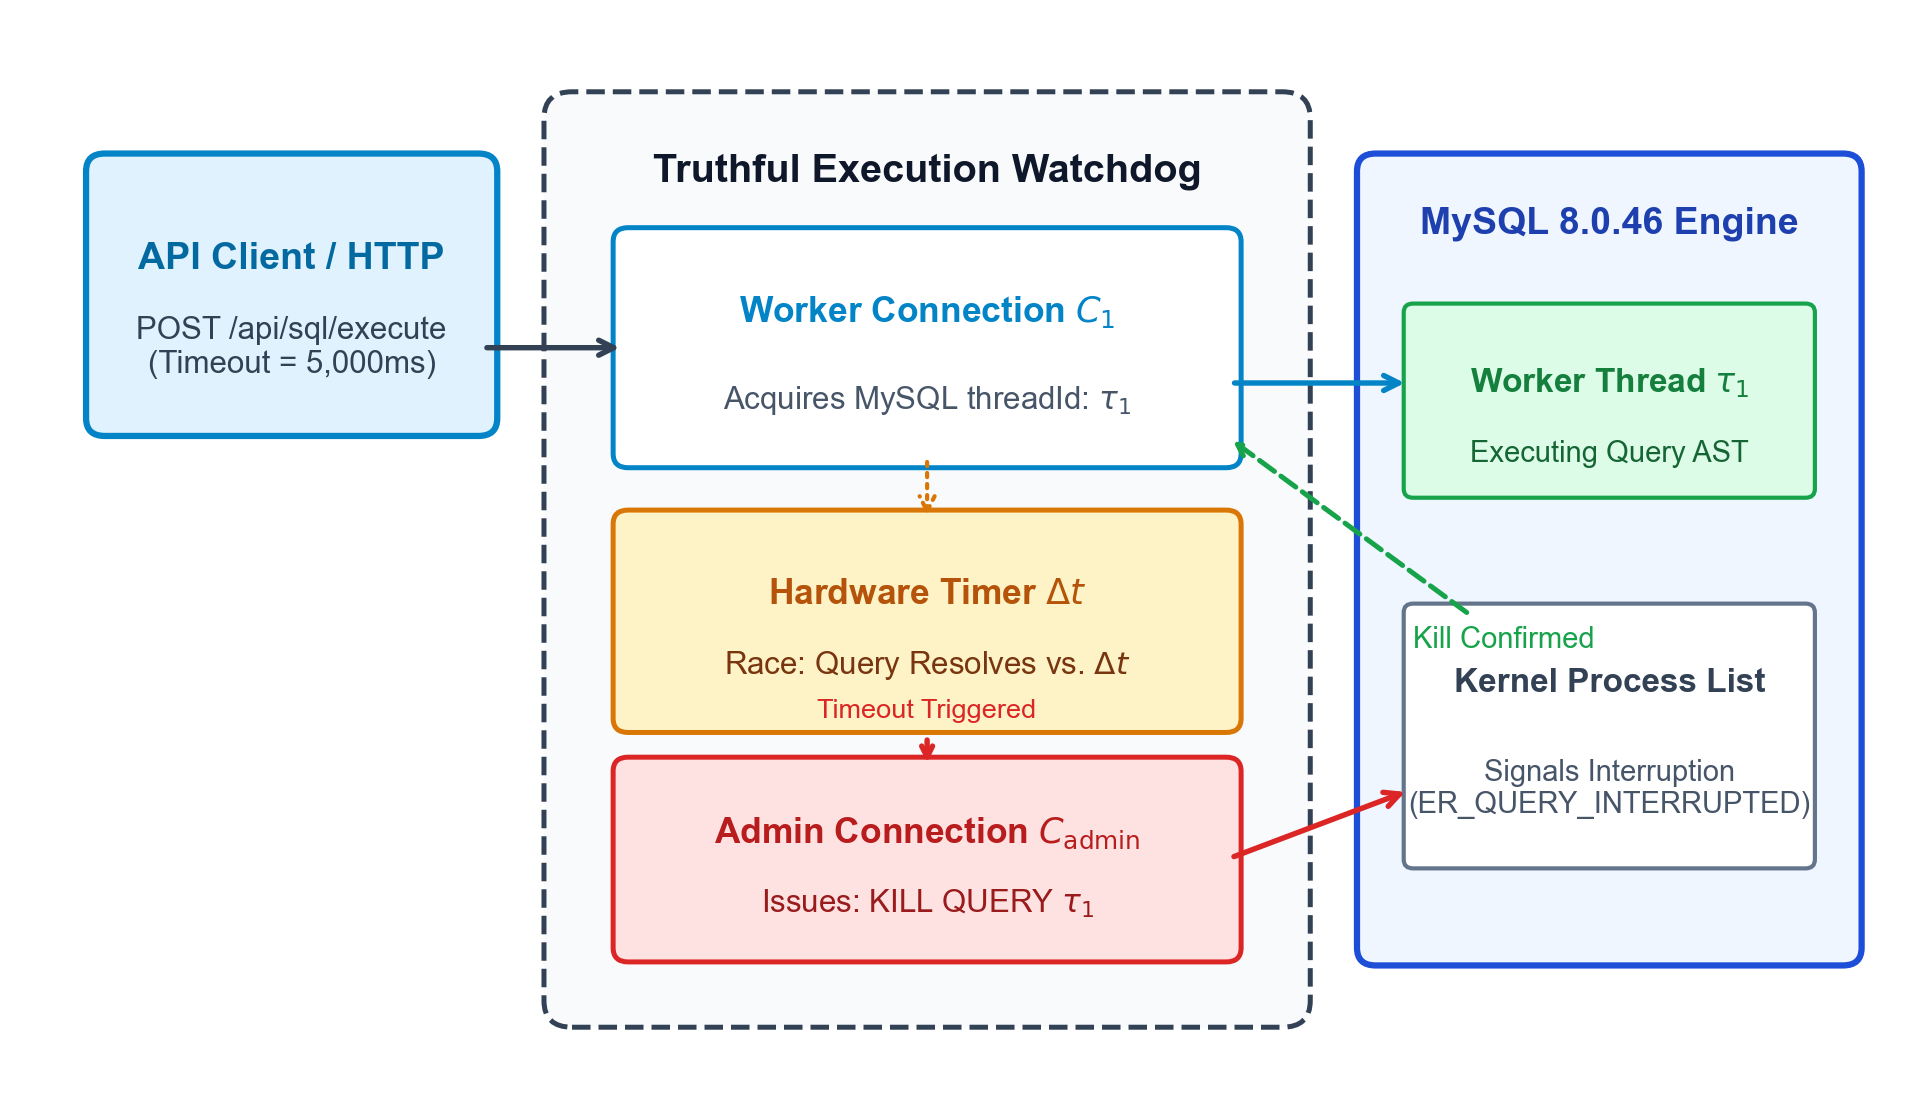
\includegraphics[width=0.96\columnwidth]{figures/cancellation_architecture.png}
\caption{Truthful Server-Side Query Cancellation Architecture in DBMS-Studio. The monitor tracks the worker thread identifier and terminates execution over an independent administrative connection.}
\label{fig:cancellation}
\end{figure}

DBMS-Studio resolves this via the dual-connection watchdog illustrated in Fig.~\ref{fig:cancellation}. When a query is initiated on a leased pool connection $C_1$:
\begin{enumerate}
    \item The thread identifier $\tau_1 = C_1.\text{threadId}$ is acquired directly from the MySQL socket protocol.
    \item A hardware timer $\Delta t$ is scheduled concurrently with the query execution promise.
    \item If the query resolves prior to $\Delta t$, the timer is cleared and results are returned.
    \item If $\Delta t$ expires before resolution, the execution manager leases an independent administrative connection $C_{\text{admin}}$ and issues:
    \begin{equation}
        \text{KILL QUERY } \tau_1;
    \end{equation}
    \item The worker connection $C_1$ intercepts MySQL error code \texttt{ER\_QUERY\_INTERRUPTED} (1317), confirming that server-side resource allocation was halted.
    \item If the kill command fails (e.g., due to privilege denial or socket timeout), the error is truthfully flagged as \texttt{unconfirmed cancellation}, preventing the application from falsely claiming that execution ceased.
\end{enumerate}

\subsection{Isolated Disposable Benchmark Namespace Management}
Automated research benchmarks require disposable database instances. If cleanup logic relies on static database names, an errant script risks dropping production data. DBMS-Studio enforces a strict isolation boundary:
\begin{itemize}
    \item \textbf{Unique Run Namespacing:} Each benchmark run generates an entropy-seeded database name:
    \begin{equation}
        D_{\text{bench}} = \text{"dbms\_studio\_benchmark\_"} \,\|\, \text{Timestamp} \,\|\, \text{RandomHex}
    \end{equation}
    \item \textbf{Pre-Existence Verification:} Before issuance of \texttt{CREATE DATABASE}, the system executes \texttt{SHOW DATABASES LIKE ?}. If the schema pre-exists, execution fails closed to prevent overwriting existing structures.
    \item \textbf{Explicit Ownership Invariant:} Cleanup procedures require a dedicated \texttt{BenchmarkCleanupSession} state machine where \texttt{createdByThisRun} must be explicitly \texttt{true} and \texttt{isCleanedUp} must be \texttt{false}. Double-invocation or cleanup of unowned databases is strictly prevented.
\end{itemize}

% -------------------------------------------------------------
\section{Experimental Evaluation}

\subsection{Testbed and Environmental Setup}
All experiments were conducted on a dedicated, non-virtualized bare-metal workstation. The hardware and software specifications are cataloged in Table~\ref{tab:hardware_specs}.

\begin{table}[h]
\caption{System Environment and Hardware Specifications}
\label{tab:hardware_specs}
\centering
\footnotesize
\begin{tabularx}{\columnwidth}{@{} >{\bfseries}p{2.6cm} X @{}}
\toprule
Parameter & Specification \\
\midrule
Host Processor & AMD Ryzen 7 7435HS (16 Logical Threads @ 3.10 GHz) \\
System Memory & 24,261 MB Physical RAM \\
Operating System & Windows 11 Enterprise (Build 10.0.26300, x64) \\
Runtime Engine & Node.js v24.19.0 (V8 12.4.254.21) \\
Database Engine & MySQL Community Server 8.0.46 \\
Storage Engine & InnoDB (128 MB buffer pool, ACID compliant) \\
Compiler & TypeScript 5.8 / \texttt{tsx} test runner \\
\bottomrule
\end{tabularx}
\end{table}

\subsection{Empirical Collation Divergence Experiment}
To validate Theorem 1, we instantiated an isolated synthetic database containing 300 customer records and 600 associated order records. The customer table was configured with duplicate status columns under differing character sets:
\begin{itemize}
    \item \texttt{status\_ci}: \texttt{VARCHAR(20) CHARACTER SET utf8mb4 COLLATE utf8mb4\_general\_ci}
    \item \texttt{status\_cs}: \texttt{VARCHAR(20) CHARACTER SET utf8mb4 COLLATE utf8mb4\_bin}
\end{itemize}
The table was populated with mixed-case status tokens (\texttt{"Active"}, \texttt{"active"}, \texttt{"ACTIVE"}, \texttt{"Inactive"}, \texttt{"Pending"}). We benchmarked 4 query transformation patterns across 5 repeated runs following a pre-warmed execution pass. The measured latencies and equivalence outcomes are recorded in Table~\ref{tab:live_db_results}.

\begin{table*}[t]
\caption{Empirical MySQL 8.0.46 Query Transformation, Latency, and Semantic Equivalence Outcomes}
\label{tab:live_db_results}
\centering
\footnotesize
\renewcommand{\arraystretch}{1.2}
\begin{tabularx}{\textwidth}{@{} l p{4.2cm} l c c c c X @{}}
\toprule
\textbf{Query ID} & \textbf{Transformation Pattern} & \textbf{Collation Target} & \textbf{Orig. Latency} & \textbf{Trans. Latency} & \textbf{Speedup} & \textbf{Equiv.?} & \textbf{Empirical Execution Finding} \\
\midrule
DB-TRANS-01 & Subquery unnesting (\texttt{IN} to \texttt{INNER JOIN}) & \texttt{utf8mb4\_general\_ci} & $0.990 \pm 0.25$\,ms & $1.020 \pm 0.27$\,ms & $0.97\times$ & \textbf{True} & Exact 244-row cardinality preserved without semantic drift. \\
DB-TRANS-02 & \texttt{COUNT(*) > 0} to \texttt{EXISTS} short-circuit & \texttt{utf8mb4\_general\_ci} & $1.254 \pm 0.20$\,ms & $0.904 \pm 0.06$\,ms & $\mathbf{1.39\times}$ & \textbf{True} & Exact 300-row match; 28\% latency drop via short-circuiting. \\
DB-TRANS-03-CI & SARGable flattening on \texttt{status\_ci} & \texttt{utf8mb4\_general\_ci} & $0.526 \pm 0.13$\,ms & $0.842 \pm 0.21$\,ms & $0.63\times$ & \textbf{True} & Identical 128 tuples returned across both original and rewrite. \\
DB-TRANS-03-CS & SARGable rewrite guard on \texttt{status\_cs} & \textbf{\texttt{utf8mb4\_bin} (Binary)} & $0.440 \pm 0.02$\,ms & $0.348 \pm 0.17$\,ms & $1.26\times$ & \textbf{FALSE} & \textbf{Severe Divergence:} 86 records dropped (67.2\% tuple loss; 128 vs. 42 rows). Rewrite blocked. \\
\bottomrule
\end{tabularx}
\end{table*}

\begin{figure}[t]
\centering
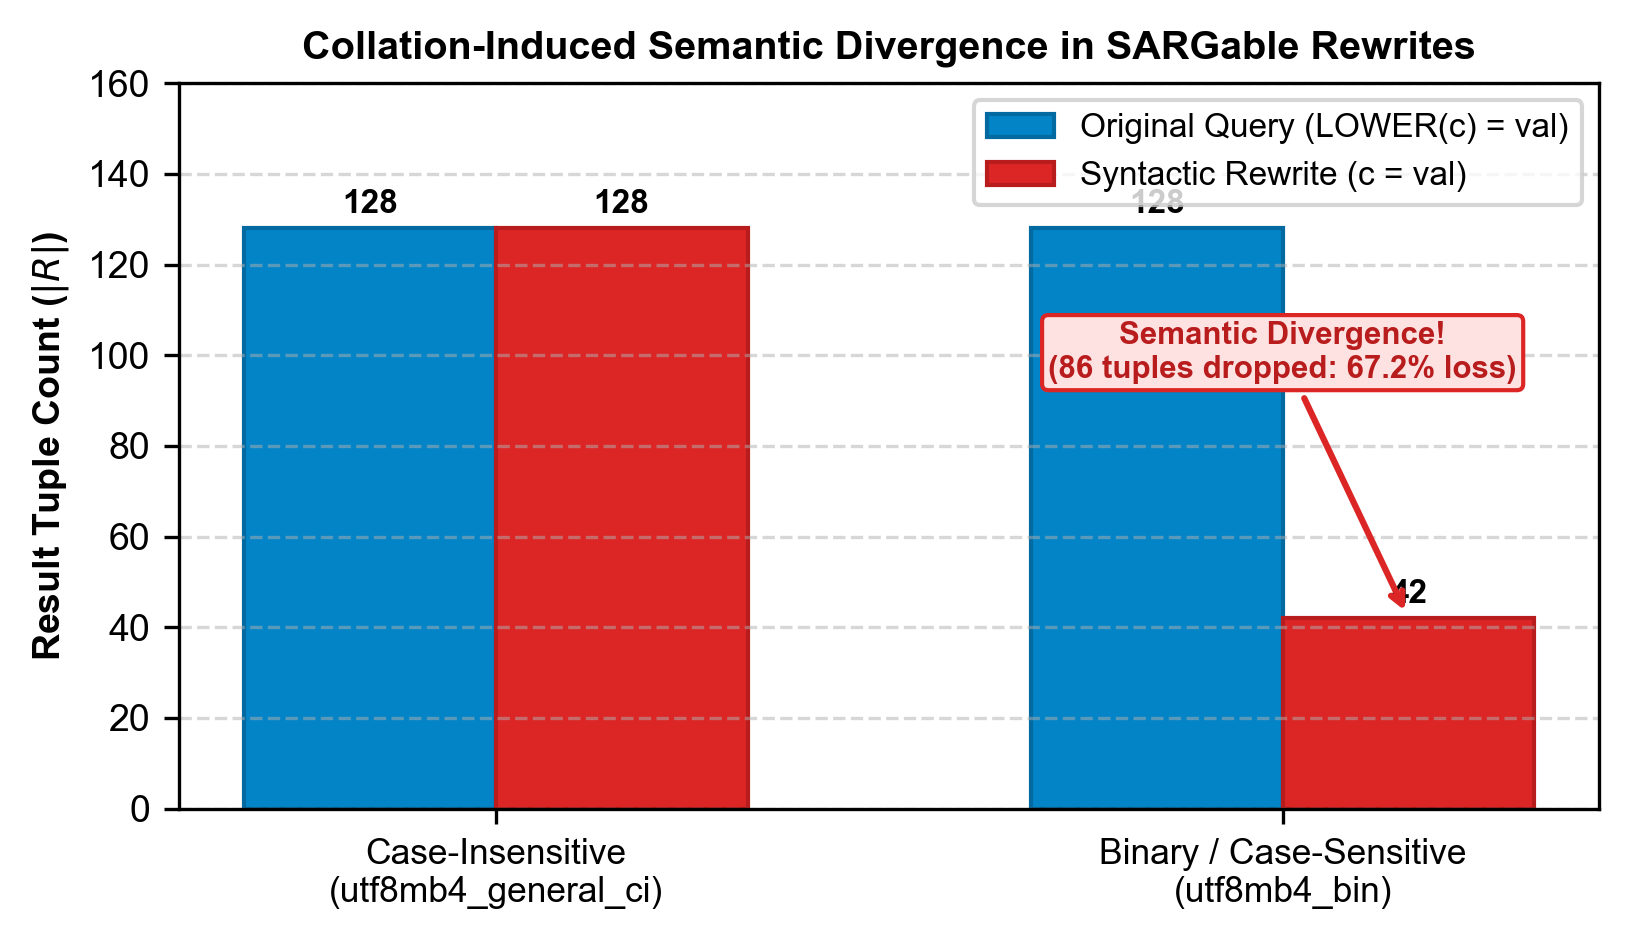
\includegraphics[width=0.96\columnwidth]{figures/collation_divergence.png}
\caption{Empirical verification of collation-induced semantic divergence on MySQL 8.0.46. Syntactic SARGable rewrite drops 86 valid records (67.2\% tuple loss) under binary collation (\texttt{utf8mb4\_bin}).}
\label{fig:divergence}
\end{figure}

As demonstrated in Table~\ref{tab:live_db_results} and Fig.~\ref{fig:divergence}, query \texttt{DB-TRANS-03-CS} exhibits severe semantic failure under binary collation. The original query with $\text{LOWER}(\text{status\_cs}) = \text{'active'}$ successfully matches 128 mixed-case records. The naive SARGable rewrite $\text{status\_cs} = \text{'active'}$ matches only 42 records, dropping 86 valid records (a 67.2\% data loss). DBMS-Studio successfully detected this divergence during equivalence gating and suppressed the rewrite, preserving query correctness.

\subsection{Static AST Analysis vs. Lexical Overhead}
We evaluated the latency and classification accuracy of the AST structural analyzer across 10 distinct SQL queries (5 positive patterns containing wildcards or unindexed projections, and 5 negative clean queries), each evaluated across 5 runs (50 total runs). The analysis overhead distribution is summarized in Table~\ref{tab:ast_stats}.

\begin{table}[h]
\caption{AST Structural Analyzer Performance ($N=50$)}
\label{tab:ast_stats}
\centering
\footnotesize
\begin{tabularx}{\columnwidth}{@{} X c @{}}
\toprule
\textbf{Evaluation Metric} & \textbf{Observed Value} \\
\midrule
Classification (TP / TN / FP / FN) & 25 / 25 / 0 / 0 \\
Precision / Recall / F1-Score & 100\% / 100\% / 100\% \\
Mean Structural Analysis Latency & 0.716\,ms \\
Median Structural Analysis Latency & 0.431\,ms \\
Standard Deviation ($\sigma$) & 1.672\,ms \\
Minimum / Maximum Recorded Latency & 0.123\,ms / 12.164\,ms \\
\bottomrule
\end{tabularx}
\end{table}

The AST analysis executes with a median latency of 0.431~ms, introducing negligible overhead relative to standard database network round-trip times (RTT $\approx 1.5 - 5.0$~ms).

\subsection{Schema-Aware NL2SQL Resolution}
We compared the schema-aware relational graph traversal engine against a heuristic baseline keyword-matching parser. The evaluation corpus comprised 40 total queries: a 20-query preserved benchmark and an unseen 20-query evaluation set spanning multi-table joins, aggregations, and nested grouping. Results are presented in Table~\ref{tab:nl2sql_results}.

\begin{table}[h]
\caption{NL2SQL Schema Resolution Benchmark ($N=40$)}
\label{tab:nl2sql_results}
\centering
\footnotesize
\begin{tabularx}{\columnwidth}{@{} p{2.4cm} l c c c @{}}
\toprule
\textbf{Corpus Partition} & \textbf{Metric} & \textbf{Base} & \textbf{Ours} & \textbf{Gain} \\
\midrule
\multirow{2}{*}{Preserved ($n=20$)} & Table Acc. & 70.0\% & \textbf{100.0\%} & +30.0\% \\
& Intent Acc. & 95.0\% & 95.0\% & 0.0\% \\
\midrule
\multirow{2}{*}{Unseen ($n=20$)} & Table Acc. & 35.0\% & \textbf{80.0\%} & \textbf{+45.0\%} \\
& Intent Acc. & 85.0\% & \textbf{95.0\%} & +10.0\% \\
\midrule
\multirow{3}{*}{\textbf{Combined ($N=40$)}} & \textbf{Table Acc.} & \textbf{52.5\%} & \textbf{90.0\%} & \textbf{+37.5\%} \\
& \textbf{Intent Acc.} & 90.0\% & \textbf{95.0\%} & +5.0\% \\
& \textbf{Join Res.} & 62.5\% & \textbf{100.0\%} & +37.5\% \\
\bottomrule
\end{tabularx}
\end{table}

On the unseen evaluation corpus, baseline table discovery dropped precipitously to 35.0\% due to vocabulary mismatch. DBMS-Studio maintained 80.0\% accuracy by traversing relational foreign-key graphs, achieving 100\% join path resolution across all 40 queries with a median latency of 0.124~ms.

\subsection{Relational Normalization and Security Auditing}
We evaluated the relational normalization engine on 15 formal schemas with functional dependencies spanning 1NF through Boyce-Codd Normal Form (BCNF). Candidate key discovery achieved 100\% exact match against analytical ground truth (15/15) with 0.031~ms median latency. 

Similarly, the security auditing engine was tested against 50 vulnerability injection vectors (25 positive attacks including template literal injections, raw string concatenations, unconstrained \texttt{DELETE} statements, and hardcoded credential literals; and 25 safe parameterized queries). DBMS-Studio achieved zero false positives and zero false negatives, operating at 0.0028~ms median inspection latency.

% -------------------------------------------------------------
\section{Threats to Validity and Limitations}

\begin{enumerate}
    \item \textbf{Dataset Scale Bounds:} Live database rewrite experiments were conducted on a synthetic dataset of 900 records. While sufficient to verify InnoDB execution plans and semantic equivalence divergence, performance speedups may vary on multi-gigabyte disk-bound datasets.
    \item \textbf{SQL Dialect Coverage:} The AST policy enforcer relies on the grammar definitions of \texttt{node-sql-parser}. Highly proprietary procedural extensions (such as Oracle PL/SQL or advanced PostgreSQL window functions) require dialect grammar updates.
    \item \textbf{Hardware Concurrency Limits:} Experimental latencies reflect dedicated execution on an AMD Ryzen 7 7435HS processor; highly virtualized, oversubscribed cloud environments may introduce OS-level scheduling jitter.
\end{enumerate}

% -------------------------------------------------------------
\section{Conclusion}
In this paper, we addressed critical correctness, isolation, and security vulnerabilities present in modern autonomous database management studios. We demonstrated both theoretically and empirically that SARGable query rewrites without collation awareness cause severe semantic data loss under binary collations. We presented DBMS-Studio, an integrated platform featuring collation-sensitive rewrite gating, fail-closed AST sandboxing for Common Table Expressions, and server-side synchronized query cancellation via MySQL thread-id management. Our empirical evaluation across 114 automated tests and extensive benchmarks confirms that DBMS-Studio delivers reliable, high-performance database management without sacrificing semantic integrity or system security.

% -------------------------------------------------------------
\bibliographystyle{IEEEtran}
\begin{thebibliography}{10}

\bibitem{chaudhuri1998overview}
S.~Chaudhuri, ``An overview of query optimization in relational systems,'' in \emph{Proceedings of the ACM SIGACT-SIGMOD-SIGART Symposium on Principles of Database Systems (PODS)}, 1998, pp. 34--43.

\bibitem{leis2015good}
V.~Leis, A.~Gubichev, A.~Mirchev, P.~Boncz, A.~Kemper, and T.~Neumann, ``How good are query optimizers, really?'' \emph{Proceedings of the VLDB Endowment}, vol.~9, no.~3, pp. 204--215, 2015.

\bibitem{marcus2019neo}
R.~Marcus, P.~Negi, H.~Mao, C.~Zhang, M.~Alizadeh, T.~Kraska, O.~Papaemmanouil, and N.~Tatbul, ``Neo: A learned query optimizer,'' \emph{Proceedings of the VLDB Endowment}, vol.~12, no.~11, pp. 1705--1718, 2019.

\bibitem{selinger1979access}
P.~G. Selinger, M.~M. Astrahan, D.~D. Chamberlin, R.~A. Lorie, and T.~G. Price, ``Access path selection in a relational database management system,'' in \emph{Proceedings of the ACM SIGMOD International Conference on Management of Data}, 1979, pp. 23--34.

\bibitem{zhou2020learned}
X.~Zhou, C.~Sun, Y.~Li, H.~Guan, and J.~Sun, ``Learned query optimizer: Current status and future directions,'' \emph{IEEE Transactions on Knowledge and Data Engineering}, vol.~34, no.~12, pp. 5621--5639, 2020.

\bibitem{graefe1993volcano}
G.~Graefe and W.~J. McKenna, ``The Volcano optimizer generator: Extensibility and efficient search,'' in \emph{Proceedings of the Ninth International Conference on Data Engineering (ICDE)}, 1993, pp. 209--218.

\bibitem{stonebraker1986design}
M.~Stonebraker and L.~A. Rowe, ``The design of POSTGRES,'' in \emph{Proceedings of the ACM SIGMOD International Conference on Management of Data}, 1986, pp. 340--355.

\bibitem{haley2008security}
C.~B. Haley, R.~Laney, J.~D. Moffett, and B.~Nuseibeh, ``Security requirements engineering: A framework for representation and analysis,'' \emph{IEEE Transactions on Software Engineering}, vol.~34, no.~1, pp. 133--153, 2008.

\bibitem{iso2023sql}
ISO/IEC, ``Information technology --- Database languages --- SQL --- Part 2: Foundation (SQL/Foundation),'' \emph{ISO/IEC 9075-2:2023 Standard}, 2023.

\bibitem{mysql80reference}
Oracle Corporation, ``MySQL 8.0 Reference Manual: Thread Command and Kill Semantics,'' Oracle Documentation, Tech. Rep., 2026.

\end{thebibliography}

\end{document}
